\section{Comunica}
\label{sec:comunica}

Comunica is een modulaire SPARQL \textit{query engine} voor het web, gemaakt door het IDLab van de universiteit Gent. Comunica is volledig open source (te vinden op github) en is beschikbaar via de npm \textit{package manager} \cite{taelman2018comunica}.

\subsection{Waarom Comunica?}
Comunica verschilt van de bestaande \textit{query processors} op verschillende niveau's. 

\subsubsection{Modulariteit}
Dankzij de hoge modulariteit van de Comunica \textit{query engine}, is het mogelijk om uitbreidingen en aanpassingen te doen op de algoritmes en functionaliteiten. Zo kan de gebruiker een op maat gemaakte \textit{engine} maken door de benodigde modules aan elkaar te koppelen aan de hand van een RDF configuratie bestand. Door dit document te publiceren kunnen experimenten ogenblikkelijk gereproduceerd worden door anderen \cite{taelman2018comunica}.

\subsubsection{Heterogene interfaces}
Heterogene interfaces binnen Comunica zorgen ervoor dat het mogelijk is om gefedereerd te queryen over heterogene bronnen. Zo wordt het bijvoorbeeld mogelijk om queries over eender welke combinatie van SPARQL \textit{endpoints}, \acrshort{tpf} \textit{interfaces}, \textit{datadumps} of andere types \textit{interfaces} te evalueren \cite{taelman2018comunica}.

\subsubsection{Webgebaseerde technologieën}
Comunica is geïmplementeerd in JavaScript (of meer specifiek TypeScript) met behulp van web gebaseerde technologieën, specifieker is het geïmplementeerd als een collectie van \textit{Node modules}. Hierbovenop heeft Comunica een \textit{test coverage} van 100\% in alle modules. Hierdoor is het mogelijk om Comunica te gebruiken in zowel browsers, de \textit{command line}, het SPARQL protocol als in gelijk welke web- of JavaScript-applicatie \cite{taelman2018comunica}.


\subsection{Design patterns}
Om het modulaire ontwerp van Comunica mogelijk te maken, zijn er verschillende ontwerppatronen gebruikt. De drie belangrijkste zullen hieronder kort besproken worden.

\subsubsection{Publish-subscribe pattern}
Het ``publish-subscribe'' patroon werkt aan de hand van messages tussen de \textit{publishers} en de \textit{subscribers}. Dit patroon doet sterk denken aan ``observer'', waarbij alle observerende entiteiten een bericht krijgen wanneer iets veranderd is van het \textit{subject} waar ze naar luisteren. Bij ``publish-subscribe'' zullen de \textit{publishers} de berichten vrijgeven naar bepaalde categorieën. De \textit{subscribers} kunnen zich dan inschrijven voor deze categorieën, waardoor ze de gepubliceerde berichten kunnen ontvangen zonder kennis te hebben over de \textit{publishers}. Het grote verschil is dan ook onmiddellijk de reden waarom er bij Comunica gekozen is voor ``publish-subscribe''. ``Publish-subscribe'' zorgt voor extra ontkoppeling tussen de verschillende software componenten waarbij er enkel kennis van de categorieën nodig is. In Comunica wordt dit patroon gebruikt om verschillende implementaties toe te staan voor bepaalde taken \cite{taelman2018comunica}.

\subsubsection{Actor model}
Het ``actor'' model is ontwikkeld om zeer parallelle systemen te bekomen. Deze systemen bestaan uit verschillende onafhankelijke agents die onderling communiceren aan de hand van \textit{messaging}. Dit is dus gelijkaardig aan het ``publish-subscribe'' patroon. Hierbij is een \textit{actor} een computationele eenheid die een specifieke taak uitvoert, die reageert op berichten en die berichten kan sturen naar andere \textit{actors}. Het voordeel hiervan is dat \textit{actors} onafhankelijk van elkaar gemaakt kunnen worden om een specifieke taak te voltooien en dat deze asynchroon afgehandeld kan worden. Zo gebruikt Comunica ook het ``actor'' model om te werken naar de hoge modulariteit. De combinatie met het ``publish-subscribe'' patroon zorgt ervoor dat elke implementatie van een bepaalde taak hoort bij een aparte \textit{actor} \cite{taelman2018comunica}.

\subsubsection{Mediator pattern}
Het ``mediator'' patroon zorgt voor een verdere reductie van de koppeling tussen software componenten die met elkaar interageren. Dankzij het ``mediator'' patroon is het ook makkelijk om de interactie tussen deze componenten aan te passen. Dit is mogelijk door het inkapselen van de interactie tussen de software componenten in een \textit{mediator} component. De software componenten zullen nu, in plaats van met elkaar de interageren, communiceren door de \textit{mediator}. Zo zijn deze componenten autonoom. Verschillende implementaties van deze \textit{mediators} zorgen voor verschillende interactieresultaten. Binnen Comunica wordt dit patroon gebruikt wanneer verschillende \textit{actors} dezelfde taak kunnen oplossen, om te beslissen welke \textit{actor} het meest geschikt is voor een taak. Eventueel kan er zelfs gekozen worden om resultaten van \textit{actors} te combineren tot één oplossing \cite{taelman2018comunica}.


\subsection{Architectuur}
Het is belangrijk om te weten dat er geen vaste ``Comunica \textit{engine}'' bestaat. Comunica is namelijk een \textit{meta engine} die geïnstantieerd kan worden in verschillende \textit{engines} gebaseerd op verschillende configuraties. Deze aanpasbaarheid wordt gerealiseerd \textit{at design-time}, gebruikmakend van \textit{dependency injection} \cite{taelman2018comunica}. 

Daarnaast is er ook een enorme flexibiliteit \textit{at run time}. Dankzij de ``publish-subscribe'', ``actor'' en ``mediator'' patronen kunnen de componenten met elkaar interageren. Dit uit zich in het ``Actor-Mediator-Bus'' patroon dat gebruikt wordt in Comunica. Dit patroon is te zien in \figureref{fig:actor-mediator-bus}. Hierin is te zien hoe een \textit{actor} een actie moet ondernemen. Deze stuurt hij vervolgens door naar de \textit{mediator}. Deze \textit{mediator} zal vervolgens een testactie sturen naar de \textit{bus}. Deze bus zal deze testactie doorsturen naar alle \textit{actors} die geregistreerd staan bij deze \textit{bus}. De \textit{bus} zal dan alle resultaten van deze testactie terugsturen naar de \textit{mediator}, waarop deze zal beslissen welke \textit{actor} het meest geschikt is voor de actie. De uiteindelijk gekozen \textit{actor} zal dan ten slotte de actie uitvoeren, zodat de \textit{mediator} het finale resultaat terug kan sturen naar de \textit{actor} die dit gehele proces heeft gestart \cite{taelman2018comunica}.

\begin{figure}
    \centering
    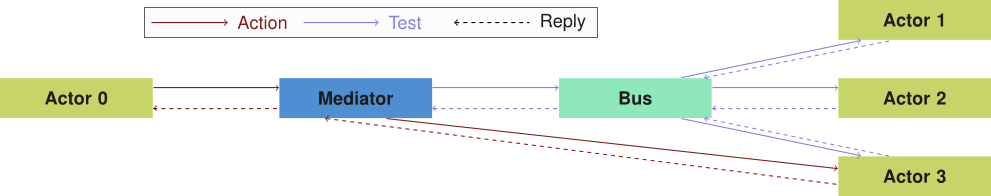
\includegraphics[width=\linewidth]{images/comunica-actor-mediator-bus.png}
    \caption{Actor-Mediator-Bus patroon, foto van ``Comunica: a Modular SPARQL Query Engine for the Web'' \cite{taelman2018comunica}.}
    \label{fig:actor-mediator-bus}
\end{figure}



\subsection{Conclusie}
Om tot een besluit te komen over Comunica kunnen er enkele feiten vastgesteld worden. Eerst en vooral kan er veel uitleg gegeven worden, maar is er gepoogd om de werking ervan duidelijk te maken op een korte, doch krachtige manier. Om de volledige en uitgebreide werking en analyse van Comunica te lezen kan best doorverwezen worden naar de officiële paper: ``Comunica: a Modular SPARQL Query Engine for the Web''. De belangrijkste punten om te onthouden zijn de vijf doelen die vooropgesteld werden bij het ontwerp van Comunica:
\begin{enumerate}
    \item \textbf{\textit{SPARQL query evaluation}}: het moet mogelijk zijn om SPARQL queries op een correcte manier te interpreteren en een resultaat weer te geven.
    \item \textbf{Modulair}: Nieuwe functionaliteiten (of bestaande functionaliteiten aanpassen) zouden slechts een minimale aanpassing aan bestaande de code mogen vereisen. Hierbij kan de gebruiker zelf kiezen welke modules hij wil inpluggen voor zijn persoonlijke \textit{engine}.
    \item \textbf{Heterogene \textit{interfaces}}: de mogelijkheid om te queryen naar verschillende soorten bronnen (zoals \acrshort{tpf} \textit{interfaces}, SPARQL \textit{endpoints} en data dumps in RDF) moet mogelijk zijn.
    \item \textbf{\textit{Federation}}: Het moet mogelijk zijn om gefedereerd te queryen. Dit betekent queryen naar verschillende bronnen. In samenhang met de heterogene \textit{interfaces} betekent dit dus queryen naar verschillende bronnen die mogelijks een verschillende soort \textit{interface} hebben.
    \item \textbf{Web gebaseerd}: Comunica is gemaakt met webtechnologieën zoals Javascript en RDF configuratie bestanden. Hierdoor kan Comunica werken in omgevingen zoals \textit{web browsers}, \textit{local} en zelfs in de \textit{command-line interface}.
\end{enumerate}